\subsubsection{Shared}

\begin{center}
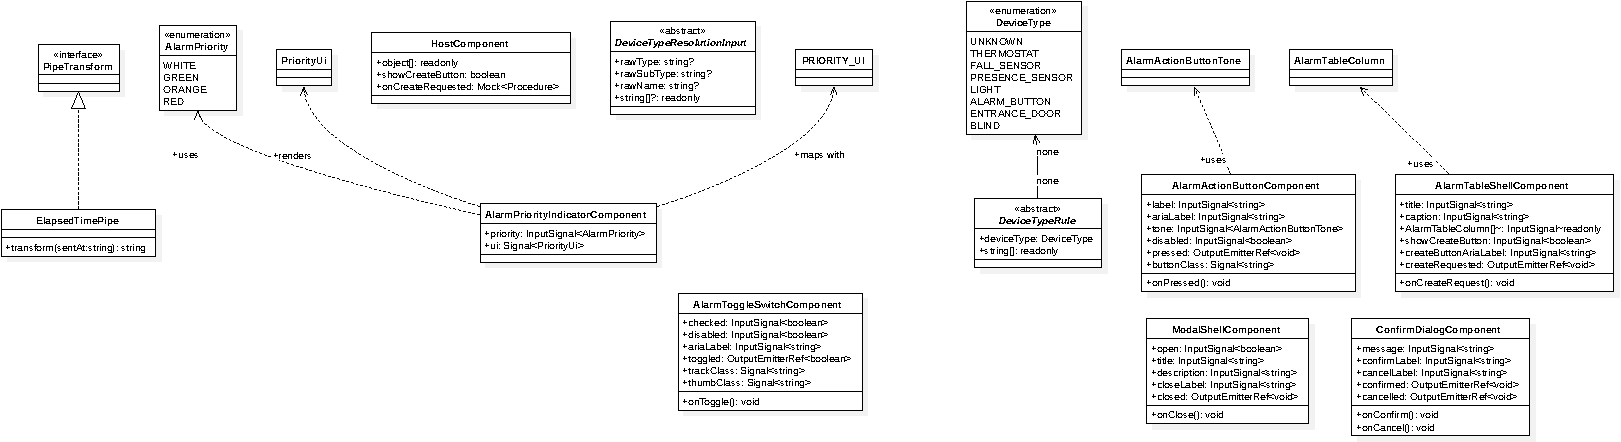
\includegraphics[width=\textwidth]{./frontend/shared/shared.pdf}
\captionof{figure}{Diagramma delle classi del modulo Shared}
\end{center}


\addAtr{+}{label: input$<$string$>$}{}
\addAtr{+}{ariaLabel: input$<$string $|$ null$>$}{}
\addAtr{+}{tone: input$<$AlarmActionButtonTone$>$}{}
\addAtr{+}{disabled: input$<$boolean$>$}{}
\addAtr{+}{pressed: output$<$void$>$}{}
\addAtr{+}{buttonClass: Signal$<$string$>$}{}
\addMet{+}{onPressed() : void}{Gestisce l'evento di interazione dell'utente emettendo il segnale di pressione solo se il componente non si trova in uno stato disabilitato.}
\makeCl{AlarmActionButtonComponent}{Componente UI riutilizzabile che rappresenta un pulsante d'azione contestuale per la gestione degli allarmi. Utilizza le Signal API di Angular per una gestione reattiva delle proprietà e calcola dinamicamente le classi CSS in base al tono visivo (neutral, danger, primary) impostato.}

\addAtr{+}{priority: input$<$AlarmPriority$>$}{}
\addAtr{+}{ui: Signal$<$PriorityUIDefinition$>$}{}
\makeCl{AlarmPriorityIndicatorComponent}{Componente visivo preposto alla rappresentazione grafica della priorità di un allarme. Attraverso l'uso di segnali reattivi (Signals), il componente mappa il valore di priorità ricevuto in input alle corrispondenti definizioni stilistiche (colori, icone, etichette) per garantire una comunicazione visiva immediata e coerente.}

\addAtr{+}{title: input$<$string$>$}{}
\addAtr{+}{caption: input$<$string$>$}{}
\addAtr{+}{columns: input$<$readonly AlarmTableColumn[]$>$}{}
\addAtr{+}{showCreateButton: input$<$boolean$>$}{}
\addAtr{+}{createButtonAriaLabel: input$<$string$>$}{}
\addAtr{+}{createRequested: output$<$void$>$}{}
\addMet{+}{onCreateRequest() : void}{Innesca l'emissione dell'evento di creazione verso il componente genitore quando l'utente interagisce con il pulsante di aggiunta.}
\makeCl{AlarmTableShellComponent}{Componente strutturale (shell) progettato per avvolgere e fornire un contesto visivo alle tabelle di gestione allarmi. Si occupa della visualizzazione del titolo, della didascalia per l'accessibilità e della gestione opzionale del punto di ingresso per la creazione di nuovi elementi, promuovendo una disposizione coerente delle interfacce tabellari.}

\addAtr{+}{checked: input$<$boolean$>$}{}
\addAtr{+}{disabled: input$<$boolean$>$}{}
\addAtr{+}{ariaLabel: input$<$string$>$}{}
\addAtr{+}{toggled: output$<$boolean$>$}{}
\addAtr{+}{trackClass: Signal$<$string$>$}{}
\addAtr{+}{thumbClass: Signal$<$string$>$}{}
\addMet{+}{onToggle() : void}{Gestisce l'evento di commutazione dello switch, invertendo lo stato corrente ed emettendo il nuovo valore tramite l'output, a condizione che il componente non sia disabilitato.}
\makeCl{AlarmToggleSwitchComponent}{Componente UI personalizzato che implementa uno switch a scorrimento (toggle) per l'attivazione o disattivazione di stati. Utilizza le Signal API per gestire in modo reattivo le classi CSS del tracciato e del cursore, garantendo feedback visivi immediati e il supporto per l'accessibilità tramite etichette ARIA.}

\addAtr{+}{message: input$<$string$>$}{}
\addAtr{+}{confirmLabel: input$<$string$>$}{}
\addAtr{+}{cancelLabel: input$<$string$>$}{}
\addAtr{+}{confirmed: output$<$void$>$}{}
\addAtr{+}{cancelled: output$<$void$>$}{}
\addMet{+}{onConfirm() : void}{Innesca l'emissione dell'evento di conferma verso il componente genitore quando l'utente accetta l'operazione.}
\addMet{+}{onCancel() : void}{Innesca l'emissione dell'evento di annullamento quando l'utente decide di chiudere il dialogo senza procedere.}
\makeCl{ConfirmDialogComponent}{Componente per la visualizzazione di una finestra di dialogo modale di conferma. Offre un'interfaccia semplice per richiedere l'approvazione dell'utente prima di procedere con operazioni potenzialmente distruttive o significative, permettendo la personalizzazione del messaggio e delle etichette dei pulsanti.}

\addAtr{+}{open: input$<$boolean$>$}{}
\addAtr{+}{title: input$<$string$>$}{}
\addAtr{+}{description: input$<$string $|$ null$>$}{}
\addAtr{+}{closeLabel: input$<$string$>$}{}
\addAtr{+}{closed: output$<$void$>$}{}
\addMet{+}{onClose() : void}{Emette il segnale di chiusura del componente per notificare al chiamante l'intenzione dell'utente di abbandonare la vista modale.}
\makeCl{ModalShellComponent}{Componente strutturale che funge da guscio per la creazione di finestre modali. Gestisce l'impalcatura visiva standard, inclusi il titolo, la descrizione opzionale e il pulsante di chiusura, permettendo di incapsulare contenuti dinamici in un contenitore coerente e accessibile.}

\addMet{+}{transform(sentAt: string) : string}{Calcola la differenza temporale tra il timestamp fornito e l'istante attuale, restituendo una stringa formattata che descrive il tempo trascorso (es. "5m fa", "2h 15m fa").}
\makeCl{ElapsedTimePipe}{Pipe personalizzata per la trasformazione di timestamp in indicatori di tempo relativo. Gestisce diverse unità di misura (secondi, minuti, ore, giorni) e include una logica di fallback per date future o non valide, facilitando la lettura dei tempi di ricezione degli eventi nell'interfaccia utente.}